\section{Findings}\label{sec:findings}

\begin{table}[t]
\centering
\caption{Results on enriching test (2024) CVEs. Systems marked $^{\diamond}$ predict CVSS scores by predicting vectors and computing the score using the CVSS formula. For each scoring method, bold highlights the best performing system and underline indicates second best. See Table~\ref{tab:main} for all results.}
\label{tab:summary}
\small
\setlength{\tabcolsep}{4pt}
\begin{tabular}{lccccc}
\toprule
System & Severity acc. & Severity macro-F1 & CWE acc. & Score MAE $\downarrow$ & Exact CVSS \\
\midrule
TF-IDF + LR & \underline{67.1} & 47.9 & \underline{67.2} & \underline{0.98} & \underline{44.1} \\
TF-IDF + CB-LR & 65.7 & \underline{51.9} & \underline{67.2} & \underline{0.98} & 40.5 \\
TF-IDF + RF & 66.9 & 47.1 & 65.2 & \underline{0.98} & 41.8 \\
Fine-tuned Phi-3.5 & \textbf{69.9} & \textbf{55.7} & \textbf{70.9} & \textbf{0.85} & \textbf{48.8} \\
\midrule
TF-IDF + LR$^{\diamond}$ & \underline{67.1} & 51.6 & \underline{67.2} & \underline{0.94} & \underline{44.1} \\
TF-IDF + CB-LR$^{\diamond}$ & \underline{67.1} & \underline{53.9} & \underline{67.2} & 0.98 & 40.5 \\
TF-IDF + RF$^{\diamond}$ & 64.0 & 47.8 & 65.2 & 1.03 & 41.8 \\
Fine-tuned Phi-3.5$^{\diamond}$ & \textbf{69.9} & \textbf{55.7} & \textbf{70.9} & \textbf{0.85} & \textbf{48.8} \\
\bottomrule
\end{tabular}
\end{table}


\paragraph{Fine-tuned Phi-3.5 performs best on all tasks.}
Table~\ref{tab:summary} summarizes test set performance (all 2024 CVEs in our snapshot of the dataset that have required information present: $n = \nTest$).
We find our fine-tuned Phi-3.5 model achieves the best performance, outperforming the TF-IDF + LR system by \nDiffLRfSev{} to \nDiffLRfVec{} points on all tasks.

\paragraph{Exact CVSS.}
Here, we consider the full eight-component vector, which is predicted for every test CVE (see Appendix~\ref{app:exact}).
In general, our models often predict similar outputs and severity, but Table~\ref{tab:agreement} shows they are frequently in disagreement.
However, for \nEitherSev\% of CVEs, at least one model is correctly predicting severity.
We next examine where and how our models err in CVSS prediction.

\begin{table}[t]
\centering
\caption{Agreement between fine-tuned Phi-3.5 and TF-IDF logistic regression (formula scoring) on the 2024 test set (\%). The last column is the share of CVEs on which at least one of the two is correct.}
\label{tab:agreement}
\small
\begin{tabular}{lccccc}
\toprule
 & Both correct & Fine-tuned only & TF-IDF only & Neither & At least one \\
\midrule
Severity & 61.3 & 8.6 & 5.9 & 24.2 & 75.8 \\
CWE & 64.4 & 6.5 & 2.9 & 26.2 & 73.8 \\
Exact CVSS vector & 39.7 & 9.1 & 4.5 & 46.7 & 53.3 \\
\bottomrule
\end{tabular}
\end{table}


First, the fine-tuned model is biased towards assigning higher scores: in CVE-2024-0003, the vulnerability is rated Critical despite its CVSS vector needing higher privileges.
Similarly, RoboDK in CVE-2024-0257 is scored lower by NIST at \nExRoboDKTrue.
In both examples the vulnerability descriptions are terse, and do not clearly explain the conditions which reduced their final scores.
Our systems defaulted to the priors learned from similar weaknesses.

Overall, the fine-tuned model outperforms all TF-IDF systems, including ridge regression.
However, there is almost no difference in performance for the fine-tuned model whether the scores are directly predicted or calculated from predicted components using the CVSS 3.1 formula.
We confirm in Table~\ref{tab:consistency} that the scores and severities produced by the CVSS formula from the fine-tuned model's predicted components are in fact almost always identical to the directly generated values.
Thus, it is apparent from its training data, which conveniently lists the CVSS components before the score, that the fine-tuned model is already acting as though calculating scores using the formula and its generated vectors.
For the logistic regression model, using formula scoring actually improves performance: score MAE decreases from \nLRdMae{} to \nLRfMae{}, and macro-F1 increases from \nLRdFone\% to \nLRfFone\% (accuracy does not change at \nLRfSev\%).
This is partly due to the increased Critical recall (\nLRdRecCritical\% $\rightarrow$ \nLRfRecCritical\%) as seen in Table~\ref{tab:tiers}, resulting from predicting Critical for \nLRfCritPred{} CVEs in comparison to \nLRfCritTrue{} in the NVD.
As such, Critical F1 increases from \nLRdFoneCritical\% to \nLRfFoneCritical\%, along with a substantial improvement in Low F1 (\nLRdFoneLow\% $\rightarrow$ \nLRfFoneLow\%).
This comes at the cost of reduced Critical precision (\nLRdCritPrec\% $\rightarrow$ \nLRfCritPrec\%).
On the other hand, random forest's comparatively worse per component performance negatively influences its formula predicted scores (\nRFdSev\% $\rightarrow$ \nRFfSev\% in accuracy and \nRFdMae{} $\rightarrow$ \nRFfMae{} MAE).

\begin{table}[t]
\centering
\caption{Recall and F1 (\%) by true severity tier on the 2024 test set.}
\label{tab:tiers}
\small
\setlength{\tabcolsep}{3.5pt}
\begin{tabular}{lcccccccc}
\toprule
 & \multicolumn{2}{c}{Critical} & \multicolumn{2}{c}{High} & \multicolumn{2}{c}{Medium} & \multicolumn{2}{c}{Low} \\
\cmidrule(lr){2-3}\cmidrule(lr){4-5}\cmidrule(lr){6-7}\cmidrule(lr){8-9}
System & Rec. & F1 & Rec. & F1 & Rec. & F1 & Rec. & F1 \\
\midrule
TF-IDF + LR, direct & 50.7 & 51.4 & 62.2 & 61.1 & 77.9 & 77.1 & 1.1 & 2.2 \\
TF-IDF + LR, formula & 73.3 & 56.1 & 62.6 & 62.6 & 71.3 & 76.8 & 6.2 & 10.9 \\
TF-IDF + LR bal., formula & 57.1 & 52.8 & 61.9 & 62.2 & 75.6 & 77.2 & 19.2 & 23.2 \\
Phi-3.5 + LoRA, formula & 76.9 & 59.7 & 63.6 & 64.6 & 75.1 & 79.0 & 11.4 & 19.6 \\
\bottomrule
\end{tabular}
\end{table}


The Low severity tier is the most difficult for all systems, likely because it represents less than 2\% of our training data.
As shown in Figure~\ref{fig:confusion}, most other errors involve predicting adjacent severity levels.
It is encouraging that using class-balanced training weights greatly improves Low tier recall to \nLRBfRecLow\% in the TF-IDF model.
The fine-tuned model performed reasonably well in this under-represented tier (recall of \nLoRAfRecLow\%) even without data rebalancing.

\begin{figure}[t]
\centering
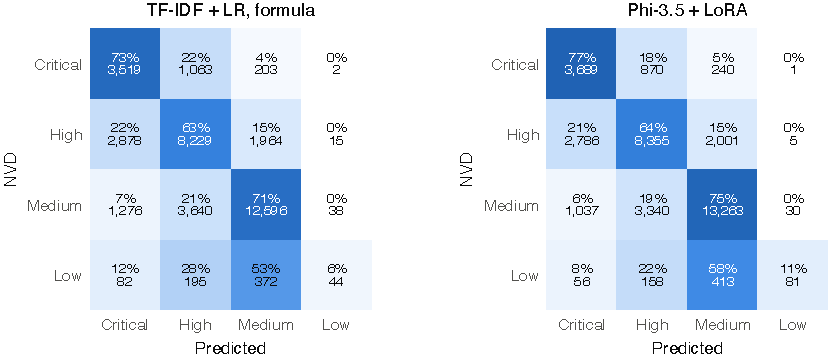
\includegraphics[width=\linewidth]{figures/fig_confusion.pdf}
\caption{Severity confusion matrices on the 2024 test set, normalized by true tier, for TF-IDF logistic regression with formula scoring (left) and fine-tuned Phi-3.5 (right).}
\label{fig:confusion}
\end{figure}

Figure~\ref{fig:components} shows per-CVSS-component accuracy on the 2024 test data, excluding the base score and severity which are dependent on the other components.
All models perform poorly on privileges required, with TF-IDF and the fine-tuned model at \nLRfCompPR\% and \nLoRAfCompPR\% respectively.
Attack complexity, scope, attack vector, and user interaction are likely easier to classify because they are almost always explicitly specified in the vulnerability description, and indeed, all systems perform well with above 90\% accuracy.
The next most difficult components after privileges required are the confidentiality, integrity, and availability impact scores, where \citet{marchiori2025canllms} found LLMs underperform embedding classifiers.
By contrast, we find that our fine-tuned model sees its largest improvements over TF-IDF on the less keyword dependent privileges required and CIA components, for instance, accuracy increases on the confidentiality and integrity components are \nLRfCompC\% $\rightarrow$ \nLoRAfCompC\% and \nLRfCompI\% $\rightarrow$ \nLoRAfCompI\% respectively.

\begin{figure}[t]
\centering
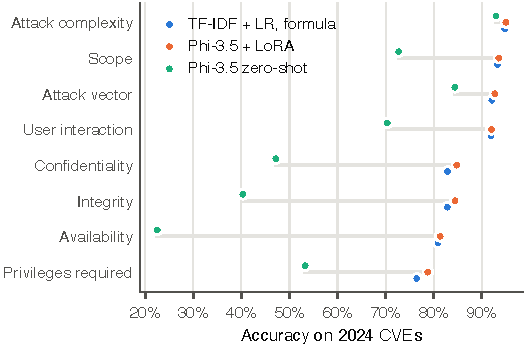
\includegraphics[width=0.62\linewidth]{figures/fig_components.pdf}
\caption{Accuracy per CVSS component on 2024 CVEs. TF-IDF and the fine-tuned model are scored on the full test set, the zero-shot model on its \nSub{}-CVE sample.}
\label{fig:components}
\end{figure}

Figure~\ref{fig:cwe} shows CWE accuracy on test set CVEs against how often each NVD-assigned CWE weakness appears in training.
Our TF-IDF model was limited to predicting on the 100 most common CWEs present in the training set, whereas the language model may predict an arbitrary textual CWE.
Accordingly, our TF-IDF model scores 0\% accuracy on the \nRareCweN{} CVEs with less commonly represented CWEs, while the fine-tuned model predicts \nLoRAfRareCwe\% correctly.
As expected, weaknesses that are common, and likely named explicitly in the vulnerability description, like cross-site scripting or SQL injection vulnerabilities, are near perfectly predicted by both of our trained models.
However, for less common weaknesses, or when the description is more general in nature, it appears our models learned associations between certain weaknesses and the severity metrics.

\begin{figure}[t]
\centering
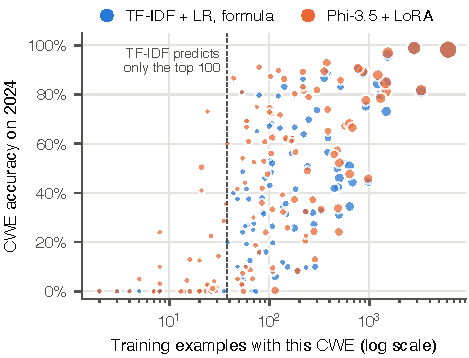
\includegraphics[width=0.62\linewidth]{figures/fig_cwe_frequency.pdf}
\caption{CWE accuracy on the 2024 test set against the number of training examples with each CWE, for every CWE with at least 20 test CVEs. Point size grows with test count.}
\label{fig:cwe}
\end{figure}

In Figure~\ref{fig:scores}, both TF-IDF and fine-tuned models over-predict the most common critical score more often than it is actually seen, likely also due to learned associations between weaknesses and common CVSS scores assigned to them.
By contrast, ridge regression predicts many scores unseen in the NVD data and does not predict the most critical or benign CVSS scores as frequently as they actually occur.
On the 2024 test set, logistic regression with formula scoring predicts a score of 9.8 (the most common critical score) on \nLRfNineEight\% of CVEs, in comparison to \nNvdNineEight\% in the NVD.
This bias results in a mean signed error of \nLRfBias, compared to only \nLRdBias{} for the ridge regression model which produces a more continuous score distribution.

\begin{figure}[t]
\centering
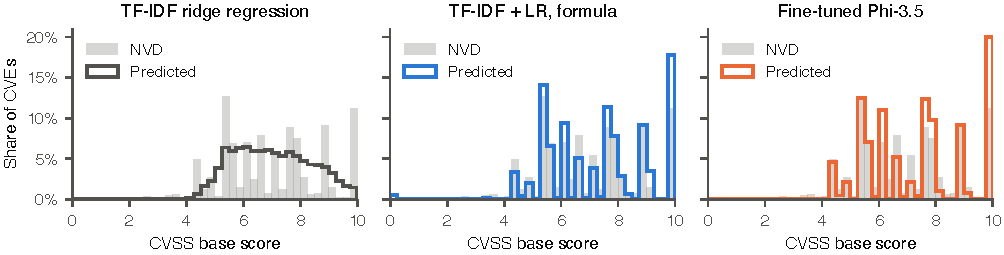
\includegraphics[width=\linewidth]{figures/fig_score_dist.pdf}
\caption{Distribution of predicted and NVD base scores on the 2024 test set in bins of 0.25, for ridge regression (left), TF-IDF logistic regression with formula scoring (middle), and the fine-tuned model (right).}
\label{fig:scores}
\end{figure}

To understand more deeply where and why models disagree with NVD-assigned vectors, we qualitatively analyzed errors.
Results are shown in Tables~\ref{tab:qualalla} through~\ref{tab:qualsomeb}: for each CVSS component, we chose four example CVEs from our 2024 test data where all (Tables~\ref{tab:qualalla} and~\ref{tab:qualallb}) or at least one (Tables~\ref{tab:qualsomea} and~\ref{tab:qualsomeb}) of our systems erred.
We bolded portions of the NVD description which may have served as clues for the true value.
In many cases only a single component differs between our predictions and the true value, and therefore exact match accuracy under-reports relative understanding of CVSS vectors.

We find the same general tendencies with the fine-tuned model as \citet{marchiori2025canllms} did with larger LLMs, namely, that some CVSS v3.1 components can be learned better than others.
Table~\ref{tab:valuefreq} compares the frequency of the possible values per CVSS v3.1 component that NIST assigned with those predicted by our model.
For example, the model overpredicts CVSS scores of 9.8 (\nLoRAfNineEight\% instead of \nNvdNineEight\%).
And correspondingly, it labels \nLoRAfCritPred{} of the CVEs from the test set as Critical, in comparison to \nLoRAfCritTrue{} CVEs labeled Critical in the NVD.
Thus, \nLoRAfCritPrec\% of those CVEs the model considers Critical are indeed Critical according to the NVD.
Overall, the model behaves similarly to the formula-scored logistic regression, meaning it is positively biased (mean signed error of \nLoRAfBias).

When analyzing the predicted vectors, we find that in \nLoRAfVecZero\% of the test CVEs, all vector components are predicted correctly (TF-IDF: \nLRfVecZero\%).
In \nLoRAfVecOne\% only one component is incorrect (TF-IDF: \nLRfVecOne\%), in \nLoRAfVecTwo\% two (TF-IDF: \nLRfVecTwo\%) and in \nLoRAfVecThreePlus\% at least three (TF-IDF: \nLRfVecThreePlus\%).
Thus, in many cases where our method misses, only one single detail is incorrectly predicted.
Often times, that detail may be hard to guess as it may be left out in the CVE description, like how exactly a DoS manifests itself (Conf.\ high or just avail.).
Also, the conditions for privilege requirements may be subtle to understand.
Overall, we can conclude that even the small fine-tuned language model significantly outperforms the classical baselines at learning how NIST enriches CVE descriptions with CVSS vectors, although the performance increase is not as big as the models sizes suggest it to be.

\begin{table}[t]
\centering
\caption{\textbf{Zero-shot Phi-3.5 trails both trained systems.} Comparison on the same random sample of 2{,}000 test CVEs. Every system is scored on exactly these CVEs.}
\label{tab:subset}
\small
\setlength{\tabcolsep}{4pt}
\begin{tabular}{lcccccc}
\toprule
 & \multicolumn{2}{c}{Severity} & CWE & Score & \multicolumn{2}{c}{Vector} \\
\cmidrule(lr){2-3}\cmidrule(lr){6-7}
System & Acc. & Macro-F1 & Acc. & MAE $\downarrow$ & Partial & Exact \\
\midrule
TF-IDF + LR, formula & 65.3\,{\scriptsize$\pm$2.1} & 47.6\,{\scriptsize$\pm$1.8} & 66.2\,{\scriptsize$\pm$2.2} & 0.99\,{\scriptsize$\pm$0.06} & 86.5\,{\scriptsize$\pm$0.7} & 42.2\,{\scriptsize$\pm$2.2} \\
Phi-3.5 zero-shot, direct & 20.8\,{\scriptsize$\pm$1.7} & 15.4\,{\scriptsize$\pm$2.4} & 25.7\,{\scriptsize$\pm$2.0} & 1.58\,{\scriptsize$\pm$0.05} & 60.5\,{\scriptsize$\pm$0.7} & 2.4\,{\scriptsize$\pm$0.6} \\
Phi-3.5 zero-shot, formula & 43.5\,{\scriptsize$\pm$2.3} & 26.8\,{\scriptsize$\pm$1.7} & 25.7\,{\scriptsize$\pm$2.0} & 2.08\,{\scriptsize$\pm$0.08} & 60.5\,{\scriptsize$\pm$0.7} & 2.4\,{\scriptsize$\pm$0.6} \\
Phi-3.5 + LoRA, formula & \textbf{69.6}\,{\scriptsize$\pm$2.0} & \textbf{52.8}\,{\scriptsize$\pm$3.3} & \textbf{68.8}\,{\scriptsize$\pm$2.1} & \textbf{0.87}\,{\scriptsize$\pm$0.05} & \textbf{87.5}\,{\scriptsize$\pm$0.7} & \textbf{48.0}\,{\scriptsize$\pm$2.1} \\
\bottomrule
\end{tabular}
\end{table}


Table~\ref{tab:subset} shows the predictions made by our zero-shot setup.
First of all, in \nZSParse\% of the cases the answer could be parsed as JSON object (from a random sample of \nSub{} CVEs, \nZSInvalid{} contained a valid JSON format but one of the CVSS components was invalid, e.g., a missing Scope value or Availability=CRITICAL).
We refer to Table~\ref{tab:zssev} for more details.
The table compares the distribution of CVSS severity written by the LLM to those that NIST derived for the same CVEs.
Clearly, the distribution is skewed towards Critical: \nZSCritShare\% of the CVEs are predicted Critical (NVD: \nSubCritShare\%) and accuracy for severity prediction is only \nZSdSev\%.
Medium is underpredicted (\nZSMediumCount{} CVEs, or \nZSMediumShare\%, instead of \nSubMediumShare\%).

Furthermore, we find that the written CVSS score is the result of the written CVSS vector in only \nZSScoreCons\% of the CVEs (see Table~\ref{tab:consistency}).
This may be due to the difficulty of performing arithmetic in context.
In fact, even for humans, CVSS calculation is considered difficult and tools exist to perform the computation.
We find similar problems when looking at the severity column of Table~\ref{tab:consistency}: here, we compare the severity label written by the LLM to the severity implied by the written score.
Only for \nZSSevCons\% they match.
Using the severity implied by the written vector instead increases the zero-shot severity accuracy on a random sample of \nSub{} test CVEs from \nZSdSev\% (using the written severity label) to \nZSfSev\%.
For comparison, on the same CVEs, fine-tuning achieves \nLoRAfSubSev\% and the TF-IDF method \nLRfSubSev\% severity accuracy.
The MAE of the scores worsens for zero-shot from \nZSdMae{} (using the written score) to \nZSfMae{} when instead calculating the score from the predicted CVSS vector.
Thus, the written scores are on average closer to the ground truth than those implied by the predicted CVSS vectors.

\begin{table}[htbp]
\centering
\caption{Self-consistency of language-model outputs (\%), where \emph{Score = formula} is the share of outputs whose written score equals the CVSS v3.1 score of the written vector and \emph{Severity = tier of score} is the share whose written severity matches the tier of the written score.}
\label{tab:consistency}
\small
\begin{tabular}{lccc}
\toprule
Model & Valid JSON & Score = formula & Severity = tier of score \\
\midrule
Phi-3.5 zero-shot & 99.7 & 3.4 & 37.0 \\
Phi-3.5 + LoRA & 100.0 & 99.8 & 100.0 \\
\bottomrule
\end{tabular}
\end{table}

